\chapter{Cluster plots of word to word models} \label{ch: appendix text model}
Visualizing matrices training with more than 500 words doesn't make sense, because the result is high dimensional and sparse. To get at least some visual feedback, \gls{mds} plots were calculated. To avoid a crowded picture, a compromise had to be made: depicting solely the \postag{} provides a manageable overview but information on single words gets lost.
\begin{figure}[H]
	\centering
		\subcaptionbox{German, ground truth \gls{mds} of word to word transitions.}{
			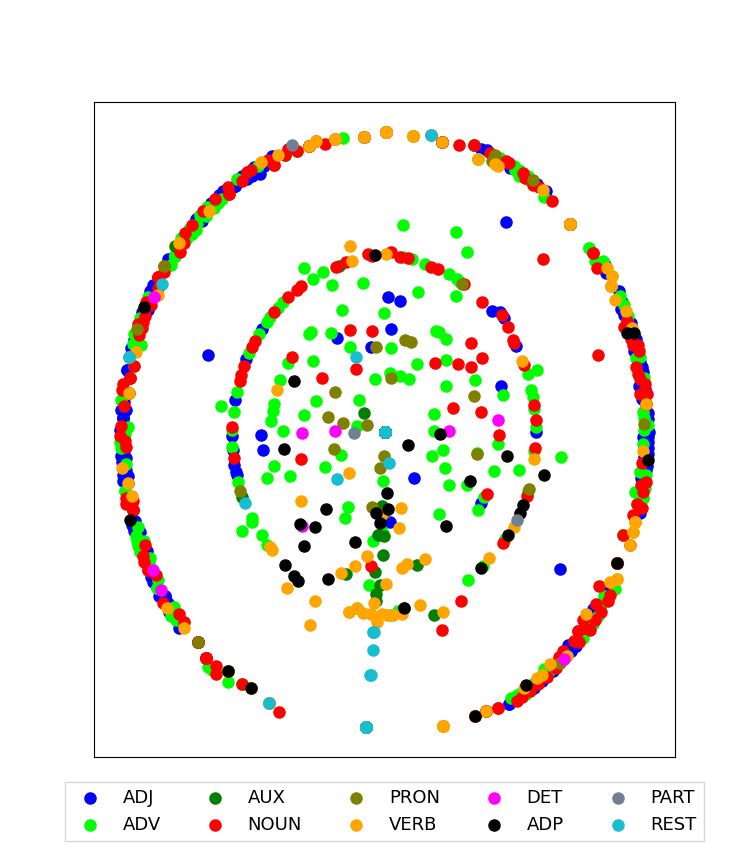
\includegraphics[width=\twocolpicwidth]{Bilder/chapter4/W2W/ground_truths/MDS_D_200pages_1500T_words.png}
		}
		\hfill
		\subcaptionbox{English, ground truth \gls{mds} of word to word transitions.\label{fig: w2w model gt en}}{
			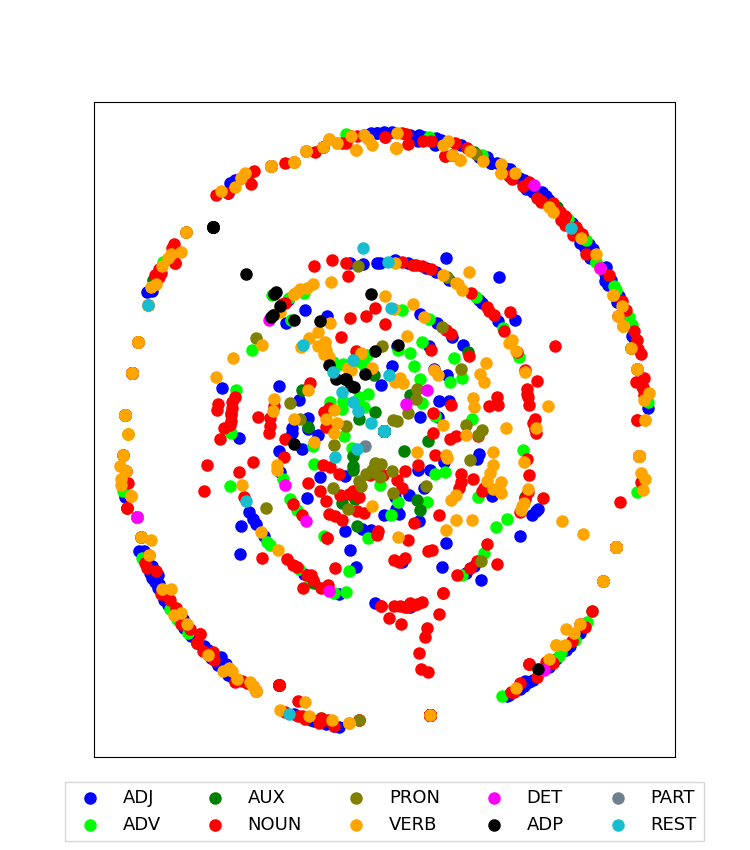
\includegraphics[width=\twocolpicwidth]{Bilder/chapter4/W2W/ground_truths/MDS_J_200pages_1500T_words.png}
		}
	\caption[]{\gls{mds} of ground truth using german and english training data.}
	\label{fig: text model gt de en mds}
\end{figure}
\begin{figure}
	\centering
		\subcaptionbox{German, \gls{mds} of learned \gls{sr} using \onehot{s}. Metric: $ 0.08 $.}{
			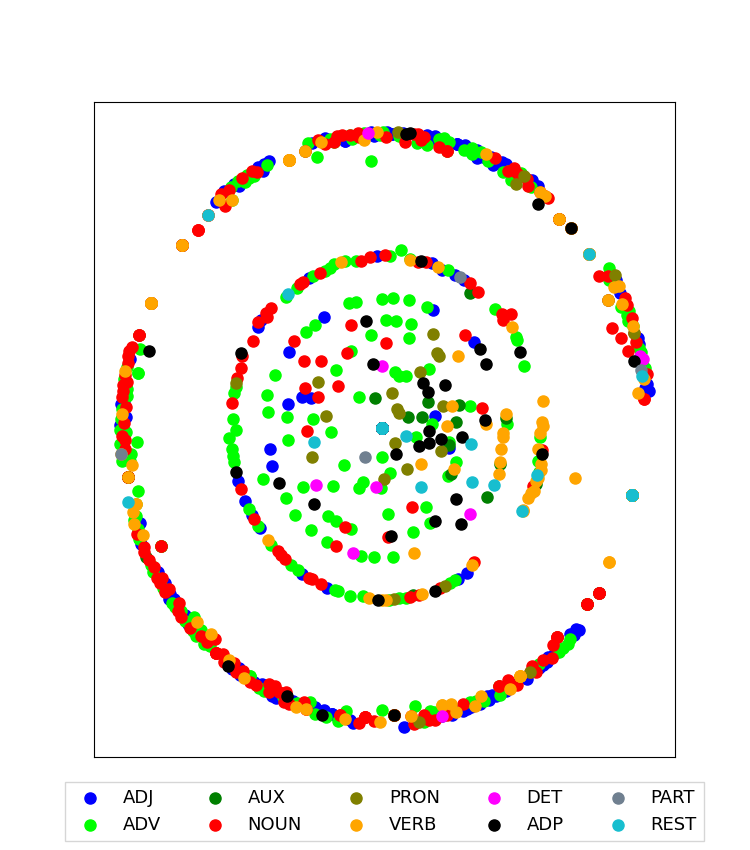
\includegraphics[width=\twocolpicwidth]{Bilder/chapter4/W2W/plots/OHE_OHE_5000E_100BS_1L_1C_200P_1500T_D/_epoch-4000/MDS_of_Transition_Probability_Matrix;_t=1,_DF=0.5.png}
		}
		\hfill
		\subcaptionbox{English, \gls{mds} of learned \gls{sr} using \onehot{s}. Metric: $ 0.1 $.}{
			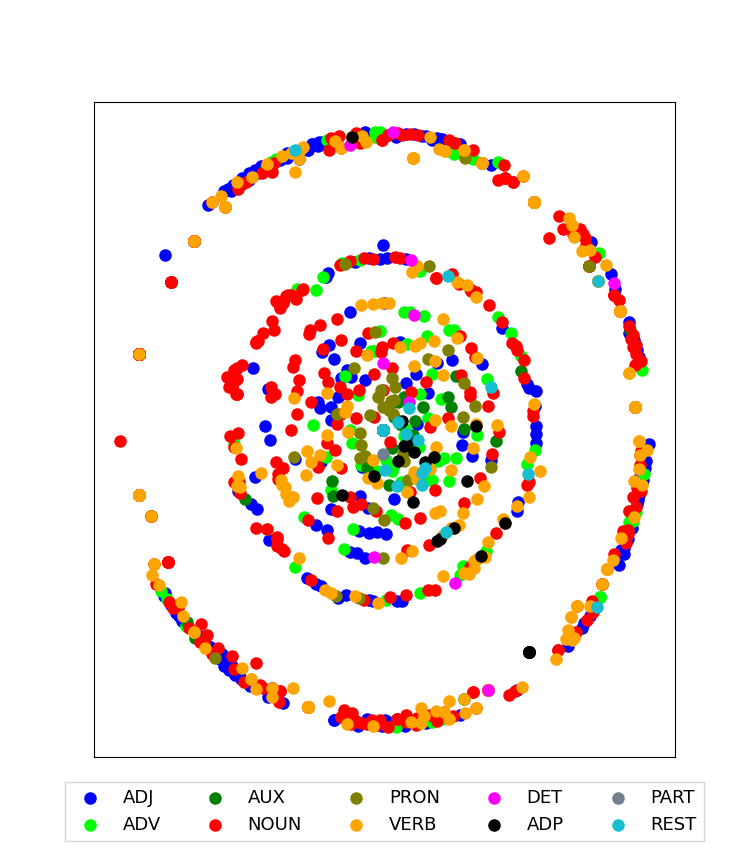
\includegraphics[width=\twocolpicwidth]{Bilder/chapter4/W2W/plots/OHE_OHE_4000E_100BS_1L_1C_200P_1500T_J/MDS_of_Transition_Probability_Matrix;_t=1,_DF=0.5.png}
		}
		\\
		\subcaptionbox{German, \gls{mds} of learned \gls{sr} using word vectors. Metric: $ 0.74 $.}{
			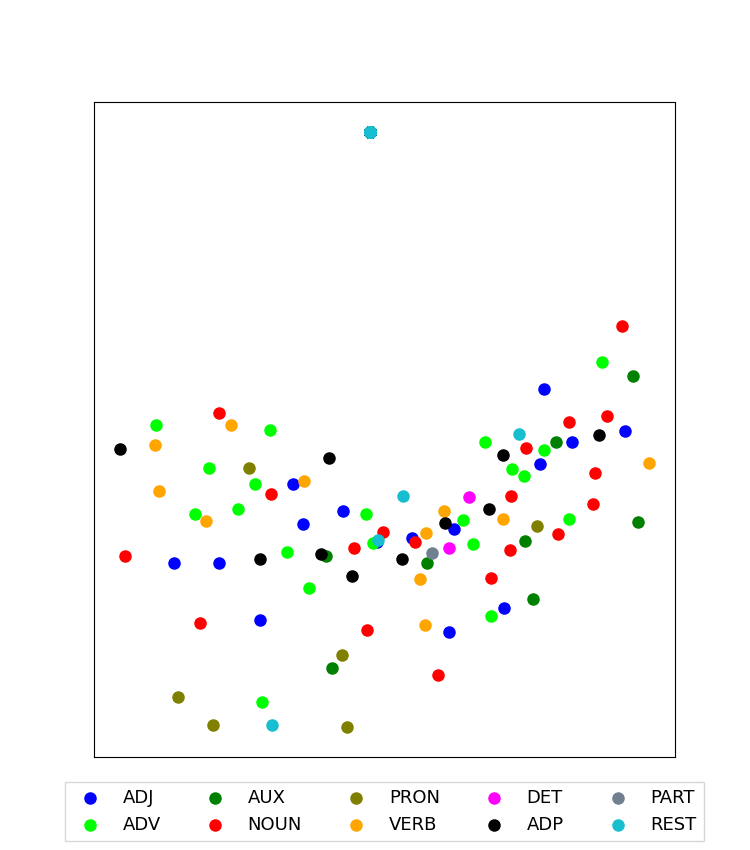
\includegraphics[width=\twocolpicwidth]{Bilder/chapter4/W2W/plots/W2V_W2V_5000E_100BS_1L_1C_200P_1500T_D/_epoch-4000/MDS_of_Transition_Probability_Matrix;_t=1,_DF=0.5.png}
		}
		\hfill
		\subcaptionbox{English, \gls{mds} of learned \gls{sr} using word vectors. Metric: $ 0.78 $.}{
			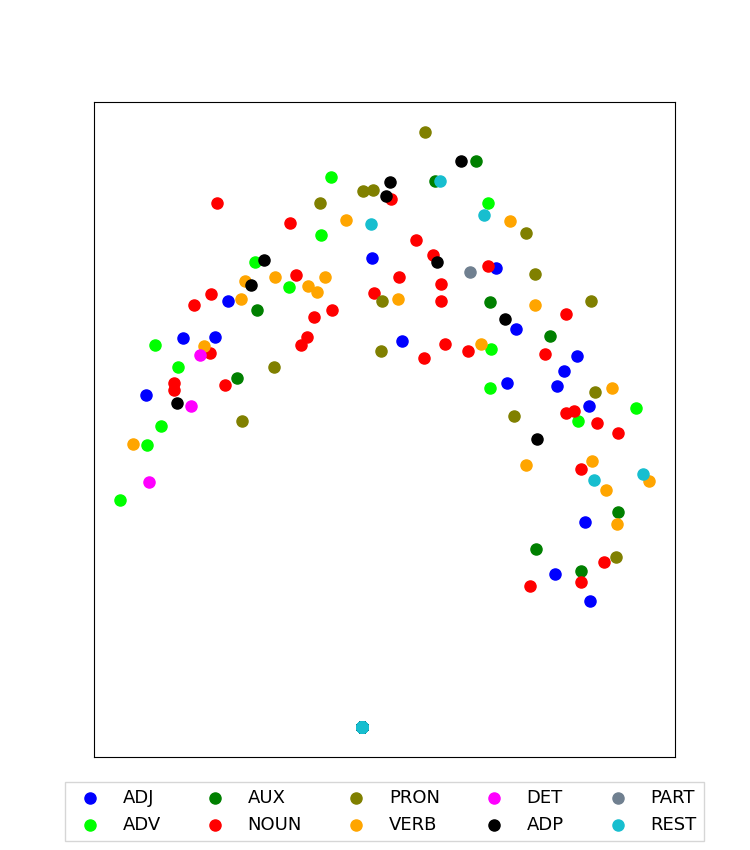
\includegraphics[width=\twocolpicwidth]{Bilder/chapter4/W2W/plots/W2V_W2V_5000E_100BS_1L_1C_200P_1500T_J/_epoch-4000/MDS_of_Transition_Probability_Matrix;_t=1,_DF=0.5.png}
		}
	\caption{The \onehot{} models show some resemblance with the ground truth in \figref{\ref{fig: text model gt de en mds}}. The disappointing results of word vectors is not just visible by the different shape the dots occupy but also by their number, much less are visible \ie many are mapped onto each other. Hence the network produces the same output for different inputs.}
	\label{fig: text model cumulativ mds plots}
\end{figure}
